上でstructをどのように定義するかご紹介しました。定義する際はフィールド名とその型が一つ一つ対応しています。実はGoは型だけの定義もサポートしています。これはフィールド名を書かない方法ではなく、匿名フィールドです。組み込みフィールドとも呼ばれます。

匿名フィールドがstructである場合、このstructがもつすべてのフィールドは隠されたまま現在定義しているこのstructに導入されます。

ひとつ例をお見せしましょう。上の説明がより具体的になります。

\begin{lstlisting}[numbers=none]
package main
import "fmt"

type Human struct {
    name string
    age int
    weight int
}

type Student struct {
    Human  // 匿名フィールド、デフォルトでStudentは
           // Humanのすべてのフィールドを含むことになります。
    speciality string
}

func main() {
    // 学生を一人初期化します。
    mark := Student{Human{"Mark", 25, 120},
                    "Computer Science"}

    // 対応するフィールドにアクセスします。
    fmt.Println("His name is ", mark.name)
    fmt.Println("His age is ", mark.age)
    fmt.Println("His weight is ", mark.weight)
    fmt.Println("His speciality is ", mark.speciality)
    // 対応するメモ情報を修正します。
    mark.speciality = "AI"
    fmt.Println("Mark changed his speciality")
    fmt.Println("His speciality is ", mark.speciality)
    // 彼の年齢情報を修正します。
    fmt.Println("Mark become old")
    mark.age = 46
    fmt.Println("His age is", mark.age)
    // 体重情報も修正します。
    fmt.Println("Mark is not an athlet anymore")
    mark.weight += 60
    fmt.Println("His weight is", mark.weight)
}
\end{lstlisting}

\begin{figure}[H]
  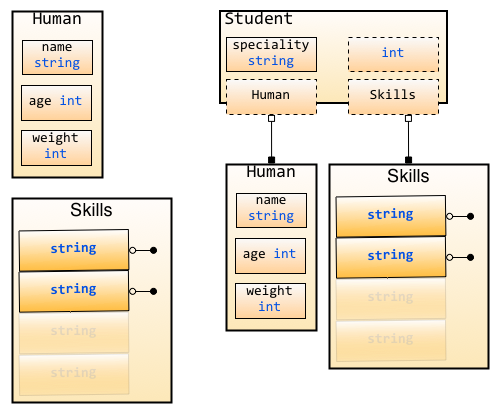
\includegraphics[width=14cm]{2.4.student_struct.png}
   \label{図2.7}
   \caption{StudentとHumanの継承方法}
\end{figure}

Studentがageとnameの属性にアクセスする際、あたかも自分のフィールドであるかのようにアクセスしたのをご覧いただけるかと思います。そうです。匿名フィールドというのはこういうものです。フィールドの継承を実現できるのです。これってクールじゃないですか?もっとクールにする方法もありますよ。studentはHumanのフィールド名でアクセスできます。下のコードを御覧ください。ほら、とってもクールでしょ?

\begin{lstlisting}[numbers=none]
mark.Human = Human{"Marcus", 55, 220}
mark.Human.age -= 1
\end{lstlisting}

匿名によるアクセスとフィールドの修正はとても便利です。でも単なるstructのフィールドですから、すべてのビルトイン型と自分で定義した型をすべて匿名フィールドとみなすことができます。下の例をご覧ください。

\begin{lstlisting}[numbers=none]
package main
import "fmt"

type Skills []string

type Human struct {
    name string
    age int
    weight int
}

type Student struct {
    Human  // 匿名フィールド、struct
    Skills // 匿名フィールド、自分で定義した型。string slice
    int    // ビルトイン型を匿名フィールドとします。
    speciality string
}

func main() {
    // 学生Jannを初期化します。
    jane := Student{Human:Human{"Jane", 35, 100},
                    speciality:"Biology"}
    // ここで対応するフィールドにアクセスしてみます。
    fmt.Println("Her name is ", jane.name)
    fmt.Println("Her age is ", jane.age)
    fmt.Println("Her weight is ", jane.weight)
    fmt.Println("Her speciality is ", jane.speciality)
    // 彼のskill技能フィールドを修正します。
    jane.Skills = []string{"anatomy"}
    fmt.Println("Her skills are ", jane.Skills)
    fmt.Println("She acquired two new ones ")
    jane.Skills = append(jane.Skills, "physics", "golang")
    fmt.Println("Her skills now are ", jane.Skills)
    // 匿名ビルトイン型のフィールドを修正します。
    jane.int = 3
    fmt.Println("Her preferred number is", jane.int)
}
\end{lstlisting}

上の例のとおり、structはstructを匿名フィールドとするだけでなく、自分で定義した型やビルトイン型も匿名フィールドとすることができます。また、対応するフィールド上で関数操作を行うこともできます(例えば例の中のappendです)。

ここで一つ疑問がでてきます:もしhumanにphoneというフィールドがあったとすると、studentもphoneと呼ばれるフィールドができます。これはどうすべきでしょうか?

Goでは簡単にこの問題を解決することができます。外側が優先的にアクセスされますので、\texttt{student.phone}とアクセスした場合studentの中のフィールドにアクセスし、humanのフィールドにはアクセスしません。

このように匿名フィールドを通じてフィールドを継承することができます。当然もしあなたが対応する匿名型のフィールドにアクセスしたくなったら、匿名フィールドの名前からアクセスすることができます。下の例をご覧ください。

\begin{lstlisting}[numbers=none]
package main
import "fmt"

type Human struct {
    name string
    age int
    phone string  // Human型がもつフィールド
}

type Employee struct {
    Human  // 匿名フィールドHuman
    speciality string
    phone string  // 社員のphoneフィールド
}

func main() {
    Bob := Employee{Human{"Bob", 34, "777-444-XXXX"},
                          "Designer", "333-222"}
    fmt.Println("Bob's work phone is:", Bob.phone)
    // もし我々がHumanのphoneフィールドにアクセスする場合は
    fmt.Println("Bob's personal phone is:",
                Bob.Human.phone)
}
\end{lstlisting}

